\documentclass{amsart}
\usepackage{graphicx}
\graphicspath{{./}}
\usepackage{hyperref}
\usepackage{csvsimple}
\usepackage{longtable}
\usepackage{epigraph}
\title{German Morals Versus Everyone Else}
\author{Zulfikar Moinuddin Ahmed}
\date{\today}
\begin{document}
\maketitle


\section{Motivation}

I was seduced by the beautiful prose of Nietzsche since I was a young teen.  I read Nietzsche in private, and it took many years before I could be confident that I understood him.  He was far from a Nazi; he was interested in artistic metaphysics and love and goodness in the end.  So I am not compelled by the bad interpreters of Nietzsche who do not see 'ubermensch' as a spiritually high and good person, not an evil power-hungry Demon.  Regardless, I was quite amazed by Nietzsche's rebellious attitude towards Christianity.  Now I was born in Bengal in 1973, and spent my life in American cities from 1987-2008 and was in Allen Texas for a decade, so I have very little idea about what Germany was like for Nietzsche.  It could be that Nietzsche just could not stand the oppressive moral pressures of nineteenth century Germany and decided to start a war with the moral Christian Germans.  The reaction is a little difficult for me to understand, because even originating from a Muslim family, I was happily an Atheist and was relatively unoppressed by religions since my mother was quite liberal and open-minded with her interest in Sufi mysticism, and my father, though absent from my teenage life was more concerned with service to the Bengali people than oppressive religious tyranny.  I have very little idea of what it is like to live in a moral deluge.  Nietzsche kept repeating that whenever there are religious forces that tyrannize man must find refuge in his private heart and so on.  That is just too difficult for me to imagine in America today.  

So I decided that I'll just roughly assume that Germany overdid the morality for centuries and do some checks to see if Germans were wise to do this.  

So I will do a compare of moral values of the world minus Germany and take a look at percent variation explained by "being German".

\section{German Acceptance of Homosexuality}

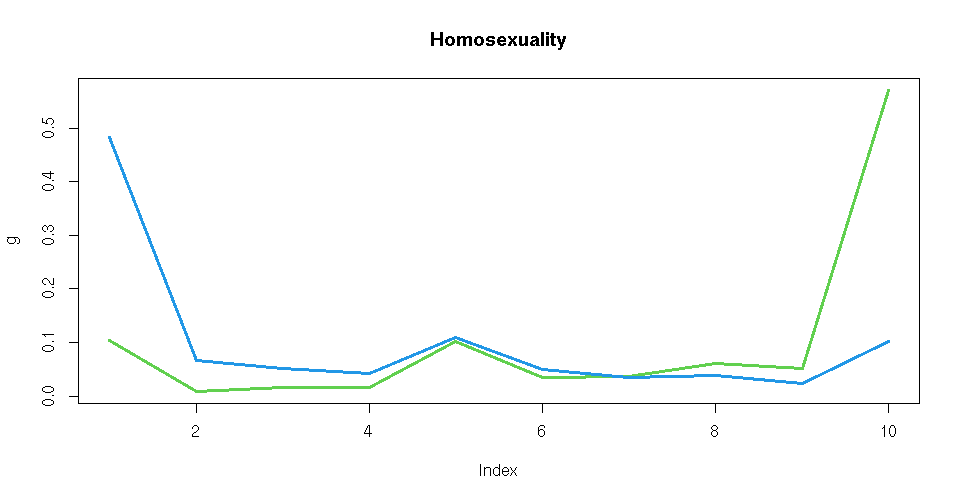
\includegraphics[scale=0.5]{gay.jpeg}

The world acceptance of homosexuality is completely different from German acceptance.  World is blue, Germans green.

\section{My Personal Views on this Matter}

I think no one has any right to interfere with the love life of anyone else.  I don't think that anyone in the world has any right to interfere with my love life.  Who I love, who I sleep with, who I like to fuck is my business and no one else's except my romantic partners and me.  Being a principled man, I believe the same is true about homosexuals.  It's their right to do whatever the fuck they want to do in their private life, and I don't get into it.

At the same time, I don't think it's a problem to believe that homosexuality is wrong.  I think people have a right to have the opinion that homosexuality is wrong.  I think it is also their right to express that opinion.  What people do not have the right to do is to transgress Natural Rights of homosexuals.  Their Life, Liberty, and Pursuit of Happiness is off limits.  So what if other people think what you are doing is wrong etc?  It does not matter.  

I do take great pride in my heterosexuality however, and consider it a grave insult to my honour to be considered homosexual.  I am heterosexual, and I do not like being considered anything but heterosexual.

\section{Sex Before Marriage}

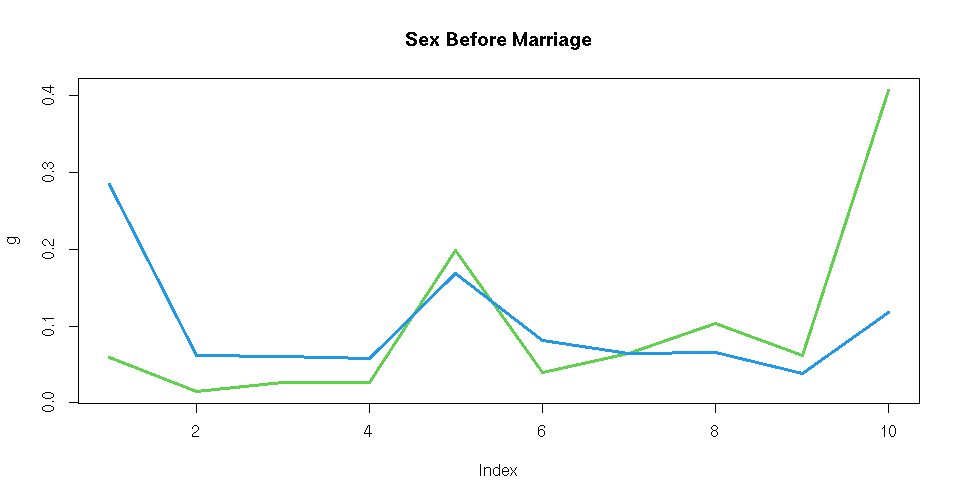
\includegraphics[scale=0.5]{sexm.jpeg}

Here Germans strongly believe sex before marriage is justified.

I have had sex before marriage myself, and so do not have strong opposition to this.  But I am extremely concerned about responsible fatherhood and strong environments for children.  I am not impressed by fatherless and single mother households with children.  I believe that fatherless children are quite ill-served by society, and also that men who are not growing with responsibilities and taking fatherhood seriously are a danger to the world.

\section{Euthanasia}

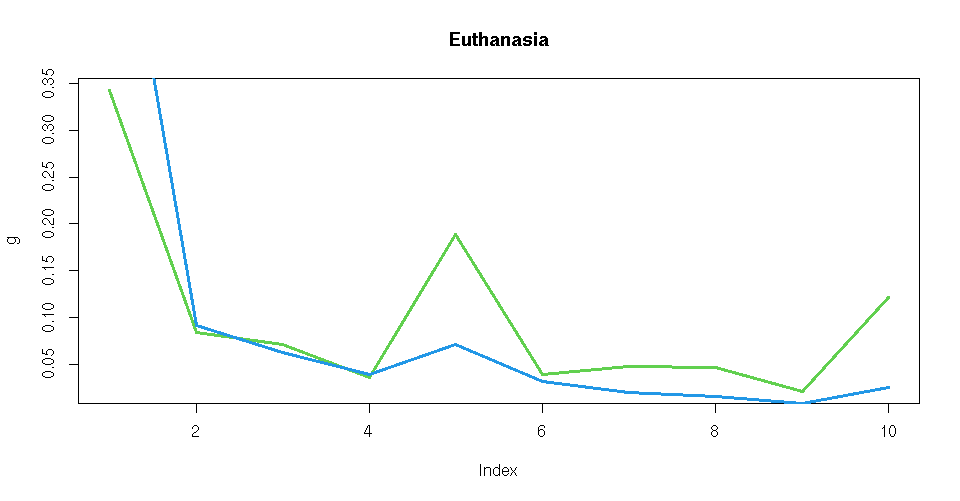
\includegraphics[scale=0.5]{euth.jpeg}

Germans are green on Euthanasia, world blue.

\section{Divorce}

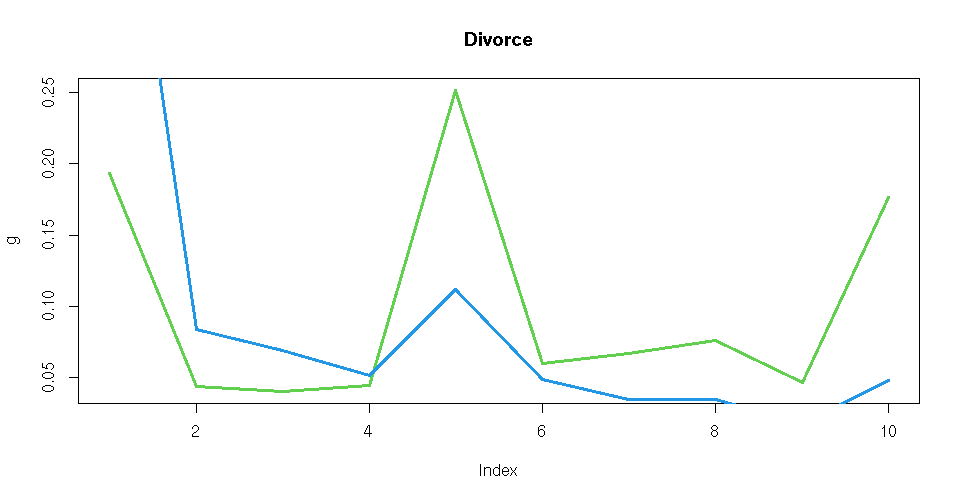
\includegraphics[scale=0.5]{divorce.jpeg}

Germans green, world blue.
I am divorced, and I think it is justified, but as I grow older, I am not interested in getting together with anyone if there is a possibility of divorce in the future.

\section{Digression: Human Nature of Human Beings is Sacred}

Human Nature developed over six million years before exodus from East Africa for non-Africans.  The evolutionary adaptations are crucial for us, and they are deep and inscrutible and complex.  The Doctor Frankensteins of meta powers, like Bill Gates, would cut and past and damage and harm Human Race but we are natural beings, humans, and cannot actually survive artificial surgery by idiots without any respect for our deep Nature.  Every human DNA is adapted for six million years of Natural Selection.  Various social consensus are idiotic by comparison.  The Human Race cannot withstand the extinction of Fatherhood; fatherhood is not an artificial institution; even the Homo Australopithecus needed paternal intervention to keep children alive, and so modern liberal dismissal of fatherhood is not enlightened but genocidal.  Children have biological needs for fathers who can give them their investment in love and guidance.  Mothers are not enough.  Liberals are insanely genocidal in producing a world which will totally destroy the human race.  Now I am generally liberal in America, but denigration of fatherhood is tantamount to denigration of Human Males altogether.  Fatherhood is an important part of male development, and has been for millions of years before Liberalism was formulated.



\end{document}